\chapter{Background and History\label{history}}
\section{Background}

\subsection{Sensor technology}
At it's core, sensors are just some photodiodes that can convert photons
into electrical charge. In this section we will cover two common sensor this is
done, as well as a brief list of pros and cons for each.

\subsubsection{Complementary Metal Oxide Semiconductor Sensors}
\textit{Complementary Metal Oxide Semiconductor} (CMOS) sensors are very old
sensors, being around since the 1960s. Over the years due to lithography
improvements they have become very good, being able to compete with with
\textit{Charged Couple Device} (CCD) sensors which are known for better image
quality technology. While CCDs have a better image quality, it requires much
more power than CMOS which can be up to 100 times less power hungry
\cite{CMOSReview}. This means that in many mobile devices and many other low
power devices wants CMOS over CCDs.

CMOS sensors are similar to the CMOS memory chips, unlike the memory chips the
sensors use photodiodes along with amplifiers \cref{fig:cmosvsccd} over
transistors. The amplifiers exist to well, amplify the signal. This design
allows us to access individual pixels quickly using random access on top of being
able to read out R, G and B signals simultaniously\cite{cmosAlen}. Because
there are so many photodiodes along with amplifiers, electrical fluctuation
is created. This causes intermittencies in the quality of the image, there are
a number of noise reduction algorithms that can be applied on the image to
remove these.

Curious readers can have a look at \cite{CMOSReview} \cite{ieeeCMOS} for a more
in depth overview of what CMOS sensors are.

\subsubsection{Charged Couple Device Sensors}
\textit{Charged Couple Device} (CCD) sensors were for a long time considered
significantly better than CMOS. It works using capacitors next to the
photodiodes to create voltage out of charge which is then read out in a serial
manner. Unlike CMOS, CDD allows you to design very small pixel sizes as the
pixels themselves don't require much real estate. The downside of this is that
this creates a lot of heat, requiring good cooling which is not always
available. In \cref{fig:cmosvsccd} we can see how the CCD sensor looks like on
a high level.

\begin{figure}
    \begin{center}
        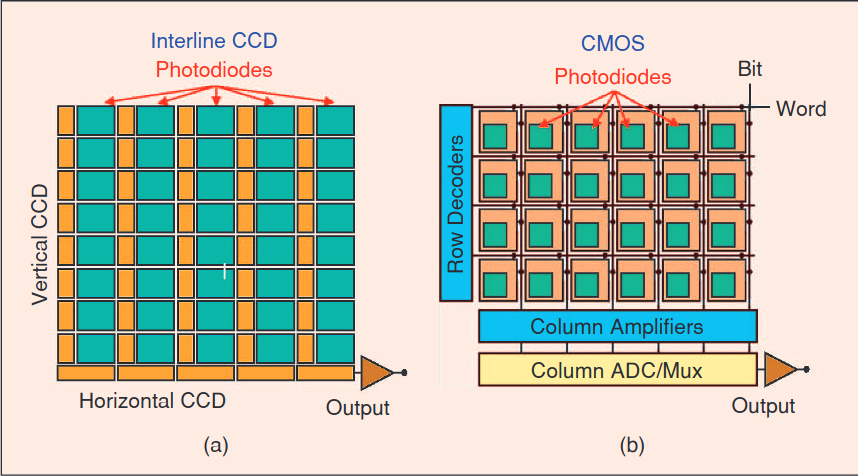
\includegraphics[width=0.55\textwidth]{figures/cmos_vs_cdd}
    \end{center}
    \caption{CMOS vs CDD comparison\cite{ieeeCMOS}}\label{fig:cmosvsccd}
\end{figure}


\subsection{Image Signal Processors}
\textit{Image Signal Processors} (ISPs) are a highly secretive piece of hardware. There
are few systems that say they even have one, and even fewer that explain how
they work. To understand how ISPs work, we will be using the Raspberry Pi
\cite{raspberrypiTuningGuide}, it is the only one that is open source (except
for the RTL code). In this section we will give an overview of what ISPs
typically do and how they function.

So ISPs, what exactly are they? As the name suggests, they process image signals.
When an image come from the sensor the signal (image) contains a lot of
redundant information. The sensor is also also not quite calibrated to the real
world environment, a lot of things are simply wrong with it. Correcting these
is an expensive process, so much so that there is a HW block in camera systems
that does this for you.

The isp has a couple steps, most work something along the lines of

\begin{enumerate}
    \item Receive raw sensor data, often a Bayer image or similar
    \item Demosaic the image, i.e. extracting the pixel data from the raw image.
          The is often done using a Bayer like filter, many exist though they
          all work in the same way.
    \item Begin the autocontrol algorithms


\end{enumerate}


\section{History}
In this section we'll largely cover the history of we've come from V4L to
libcamera.

In the early days cameras were quite simple, there effectively was just the
"press button" followed by receiving a picture. This process did not allow for
much customization. This was the case with most cameras such as webcams where
the camera sensors were "smart sensors". This meant that the cameras had a small
ISP integrated into them, they could do the processing internally. Even the
integrated laptop ones were just USB devices that spit out images. Linux had
initially had lacking support for this, but in the early 2000s Video For Linux
(V4L, later V4L2 for version 2) was developed. This covered most of the use
cases at the time.

% TODO: cite frankencamera
In 2009 the Nokia N900 was released, this was a Linux based phone that was not
like most cameras at the time. It provided interfaces for customizing just
about everything. From ISPs to Image Processing Algorithms (IPA's), this meant
that the current way camera API's worked was no longer sufficient. Enter
Frankencamera\cite{adams2010frankencamera}; this was an effort at the time
to create an API that allowed the user to express the different options that
cameras needed.
